%% LyX 2.3.6.1 created this file.  For more info, see http://www.lyx.org/.
%% Do not edit unless you really know what you are doing.
\documentclass[english]{article}
\usepackage[T1]{fontenc}
\usepackage[latin9]{inputenc}
\usepackage{color}
\usepackage{units}
\usepackage{amsmath}
\usepackage{graphicx}
\usepackage{babel}
\begin{document}

\section{Summary}
\begin{itemize}
\item vEB tree and operations
\item Direct addressing with superimposed tree of constant height
\begin{itemize}
\item Summary
\item Cluster
\item Successor and Predecessor direct addressing
\end{itemize}
\item Proto van Emde Boas tree
\begin{itemize}
\item Recursive structure
\item Successor operation 
\item Successor recurrence and running time
\item Problems with the successor operation
\end{itemize}
\item van Emde Boas Tree
\begin{itemize}
\item Recursive structure difference from proto vEB
\item Successor operation
\item Recurrence and running time
\end{itemize}
\item Reflection between proto vEB and vEB
\end{itemize}


\section{Detailed summary}

The van Embde Boas trees is tree structure that supports the dynamic
set operations: \emph{search, insert, delete, minimum, maximum, predecessor
and successor. }I will assume that duplicate keys are not allowed
so instead of the \emph{search} operation a simplified \emph{member
}operation that simply returns a boolean value will be used. Each
operation runs in $O(\lg\lg u$) time where $u$ is the size of the
universe.

Like in the book, i will go over some preliminary tree structures
until I arrive at the van Embde Boas tree, and assume that that the
universe size in an exact power of $2$. That is, $u=2^{k}$for some
integer $k\ge1$.

\subsection{Direct addressing}

In plain direct addressing we store the dynamic set as a bit vector
of length $u$, where bit $u[i]=1$ if key $i$ is in the set and
0 otherwise. If we assume we have a universe of size $u=2^{2k}$for
some integer $k$, then we will always have that $\text{\ensuremath{\sqrt{u}=\sqrt{2^{2k}}=2\sqrt{k}} is still an integer}$.
A tree of degree $\sqrt{u}$ is then superimposed over the direct
addressing scheme with height 2. Each internal node of this tree stores
the logical \textbf{or }of its children. Hence the root is only $1$if
any of the children have any members. The leaves of the tree is the
original direct addressing bit-array. \textcolor{red}{TODO: why does
this always have depth 2?}

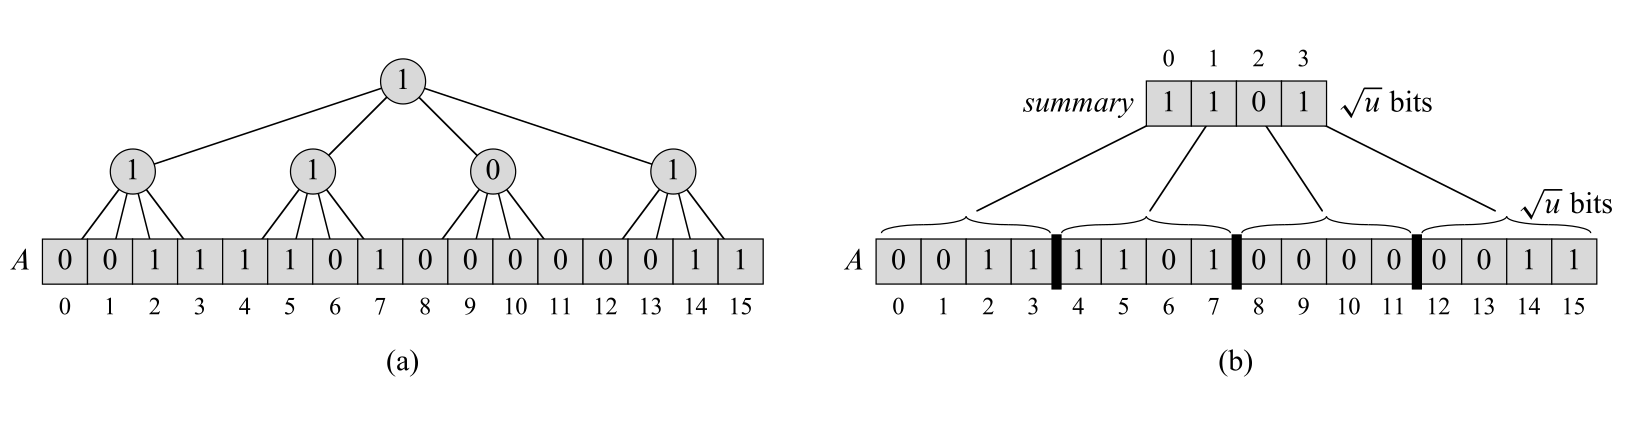
\includegraphics[width=1\linewidth]{directAddressing}

Since the $\sqrt{u}$ internal nodes are the logical or of their children,
we can think of of each internal node as holding a summary of their
$\sqrt{u}$children. Therefore, we can think of the internal nodes
as a summary bit-array of length $\sqrt{u}$bits, $summary[0,...,\sqrt{u}-1]$.
This means that $summary[i]=1$ if the sub-array $A[i\sqrt{u},...,(i+1)\sqrt{u}$
contains any elements. This sub array will be referred to as a cluster.

\textbf{Successor(x) and predecessor: }Assuming that $x$ is in the
tree. Search to the right of $x$in the cluster of $x$ until a $1$is
found(the position is the successor). In case there is nothing, then
calculate $i=\lfloor\nicefrac{x}{\text{\ensuremath{\sqrt{u}}}}\rfloor$(which
is the cluster of $x$). Then search for a $1$ to the right of $i$
in the summary buffer until a $1$ is found. This gives the index
of the cluster. Search through the cluster to find the first 1. The
predecessor is almost the same. 

In the worst case, we search through two clusters of size $\sqrt{u}$and
the summary buffer of size $\sqrt{u}$. Therefore, successor and predecessor
take \textbf{$O(\sqrt{u})$ }. 

\subsection{Proto van Embde Boas}

For this tree structure we assume that the universe size $u=2{{}^2}^{k}$
for some integer $k$. We expand the previous tree structure further
by making it recursive. We start by making a (summary) structure of
size $\sqrt{u}=u^{\nicefrac{1}{2}}$where each item holds $u^{\nicefrac{1}{4}}$items.
Each of the $u^{\nicefrac{1}{4}}$items holds structures of $u^{\nicefrac{1}{8}}$items
and so on until we reach a structure of $2$ items.

Let us say our universe is 64-bit numbers. Then we have $u=2^{64}$
and a \textbf{$\log u=\log2^{64}=64$}-bit key $x$. From the simple
direct addressing with a $\sqrt{u}$ -degree superimposed tree, we
got the cluster number by
\[
cluster=\lfloor\nicefrac{x}{\sqrt{u}\rfloor}
\]

and if $x$ is a $\lg u$-bit number, then we by get the cluster number
by the $\nicefrac{\lg u}{2}$ most important bits. Within the cluster,
$x$ appear as the index given by the lower $\lg u/2$ bits. These
are calculated by $x\mod\sqrt{u}$. We index the different bits by

\[
high(x)=\lfloor\nicefrac{x}{\sqrt{u}\rfloor}
\]
\[
low(x)=x\mod\sqrt{u}
\]
\[
index(x,y)=x\sqrt{u}+y
\]

Where the $index$ function builds a number, treating $x$ as the
upper half bits and $y$ as the lower half numbers.
\end{document}
